\documentclass[11pt]{article}


\marginparwidth 0.5in 
\oddsidemargin 0.25in 
\evensidemargin 0.25in 
\marginparsep 0.25in
\topmargin 0.25in 
\textwidth 6in \textheight 8 in

\usepackage{multirow}
\usepackage{tabularx}
\usepackage{longtable}
\usepackage[utf8]{inputenc}
\usepackage[spanish]{babel}
\usepackage{graphicx}
\usepackage{wrapfig}


\begin{document}
\author{Diego Andai Castilla}
\title{Reporte de gases contaminantes}
\maketitle

\section{Resumen}

En el siguiente informe se presenta el análisis estadístico de la cantidad de gases contaminantes en 59 ciudades de EE.UU. y su relación con distintas variables como mortalidad, temperatura, densidad poblacional, ingresos medios, entre otras.

Los gases contaminantes a estudiar son:

\begin{itemize}
    \item NOx: óxidos de nitrógeno, generados por combustión a altas temperaturas.
    \item HC: hidrocarburos, compuestos de carbono e hidrógeno derivados del petróleo.
    \item SO2: dióxido de azufre, tambien causado por la combustión.
\end{itemize}

Todos estos son perjudiciales para la salud de los ciudadanos y están relacionados con la utilización de derivados del petróleo en procesos de combustión, como por ejemplo lo que ocurre en los motores de los autos. La abreviación que se muestra arriba será utilizada en este informe.

\section{Variables a estudiar}

A continuación se presenta una descripción estadística de las distintas variables a considerar en el estudio.

\subsection{Gases contaminantes}

\subsubsection{NO_x}

\begin{center}
\begin{tabular}{|c|c|}
    \hline
    Variable & Unidad  \\ \hline
    NO_x & ppm \\
    \hline
\end{tabular}
\end{center}

\textbf{Medidas descriptivas de centro:}

\begin{center}
\begin{tabular}{|c|c|c|}
    \hline
    Promedio ponderado & Mediana & Moda \\ \hline
    22.9661 & 9 & 4 \\
    \hline
\end{tabular}
\end{center}

Como podemos observar, la cantidad de NOx en el aire tiene gran asimetría. Sus medidas centrales están muy separadas por lo que probablemente existan outliers que estén arrastrando el promedio hacia valores mayores. Esperamos encontrar ciertas ciudades que se escapen de las demás, estas son San Francisco (NOx: 171[ppm]) y Los Ángeles - Long Beach (NOx: 319[ppm]).
\\
\\
\textbf{Medidas descriptivas de posición:}

\begin{center}
\begin{tabular}{|c|c|c|c|c|}
    \hline
    Mínimo valor & Primer cuartil & Segundo cuartil & Tercer cuartil & Máximo valor\\ \hline
    1 & 4 & 9 & 24.5 & 319\\
    \hline
\end{tabular}
\end{center}

Comprobamos la idea anterior, el 75\% de los datos se encuentra antes de los 24.5[ppm].
\\
\\
\textbf{Medidas descriptivas de dispersión y forma:}

\begin{center}
\begin{tabular}{|c|c|c|c|c|}
    \hline
    Desviación estándar  & Varianza & Skewness & Kurtosis\\ \hline
    46.6657 & 2177.689 & 4.8685 & 26.2062\\
    \hline
\end{tabular}
\end{center}

Por último, encontramos que las medidas de dispersión confirman nuestra hipótesis, la medida de skewness es positiva asi que la mayor densidad de datos está a la izquierda. La kurtosis a su vez nos indica que la forma de la distribución será puntiaguda, ya que tenemos la cola derecha con valores muy lejanos a la media.
\\
\\
\textbf{Gráficos de distribución:}
\\

\begin{wrapfigure}{r}{0.5\textwidth}
    \centering
    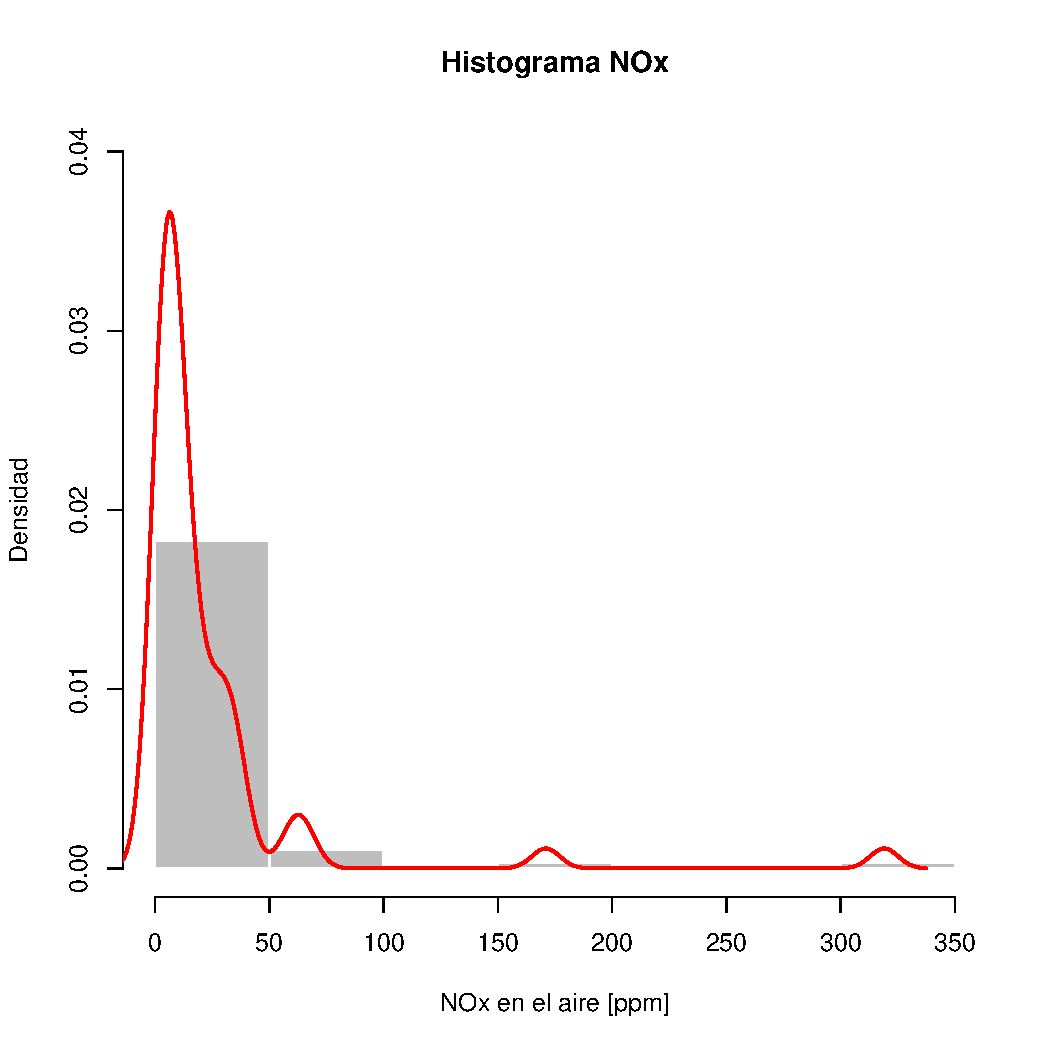
\includegraphics[width = 0.4\textwidth]{histnox}
\end{wrapfigure}

En el histograma de densidad, podemos observar todo lo que esperábamos. Un gráfico cargado a la izquierda, por esto la medida de skewness nos arrojó un valor positivo. Existe un par de valores que se escapan de la densidad general, justamente los que mencionamos en las medidas centrales. La mayoría de los datos se encuentran antes de los 50[ppm]. Podemos apreciar gráficamente la medida de kurtosis, en la punta del gráfico. 
\\
\\
\\
\\

\begin{wrapfigure}{l}{0.5\textwidth}
    \centering
    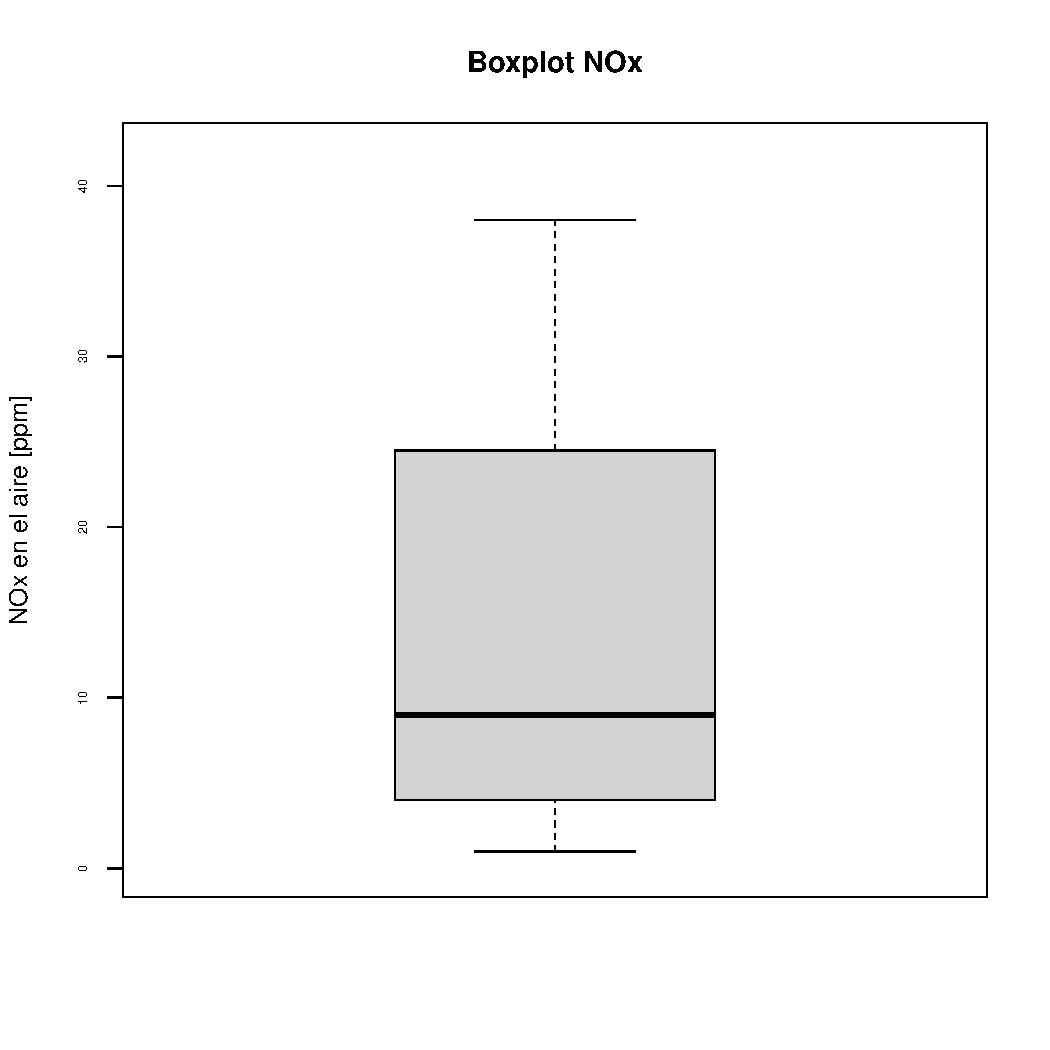
\includegraphics[width = 0.4\textwidth]{boxnox}
\end{wrapfigure}

Por último, el boxplot de los datos acota la mayor parte de su distribución antes de los 40[ppm]. Esto será algo a considerar más adelante cuando comparemos estos datos con otras variables. 

En definitiva, la variable de NOx si bien tiene algunos outliers, se concentra entre 1[ppm] y 40[ppm]
\\
\\
\\
\\
\\
\\

\subsubsection{HC}

\begin{center}
\begin{tabular}{|c|c|}
    \hline
    Variable & Unidad  \\ \hline
    HC & ppm \\
    \hline
\end{tabular}
\end{center}

\textbf{Medidas descriptivas de centro:}

\begin{center}
\begin{tabular}{|c|c|c|}
    \hline
    Promedio ponderado & Mediana & Moda \\ \hline
    38.4746 & 15 & 6 \\
    \hline
\end{tabular}
\end{center}

Al igual que los niveles de NOx, los niveles de HC en el aire presentan asimetría, juzgando los valores de medida central. De nuevo observamos que San Francisco (HC: 311[ppm]) y Los Ángeles-Long Beach (HC: 648[ppm]) se escapan bastante de los valores medios, y pueden ser considerados como outliers.
\\
\\
\textbf{Medidas descriptivas de posición:}

\begin{center}
\begin{tabular}{|c|c|c|c|c|}
    \hline
    Mínimo valor & Primer cuartil & Segundo cuartil & Tercer cuartil & Máximo valor\\ \hline
    1 & 7 & 15 & 30.5 & 648\\
    \hline
\end{tabular}
\end{center}

Comprobamos la idea anterior, el 75\% de los datos se encuentra antes de los 30.5[ppm].
\\
\\
\textbf{Medidas descriptivas de dispersión y forma:}

\begin{center}
\begin{tabular}{|c|c|c|c|c|}
    \hline
    Desviación estándar  & Varianza & Skewness & Kurtosis\\ \hline
    92.6388 & 8581.943 & 5.2732 & 30.0754\\
    \hline
\end{tabular}
\end{center}

Encontramos que las medidas de dispersión confirman nuestra hipótesis, esta variable tiene una dispersión y asimetría incluso mayor a la anterior, esto obviamente debido a que los valores que se escapan son incluso mayores a los que se escapan en la cantidad de NOx. La kurtosis es también mayor y por lo tanto de nuevo esperamos una forma puntiaguda en la línea de densidad.
\\
\\
\textbf{Gráficos de distribución:}
\\

\begin{wrapfigure}{r}{0.5\textwidth}
    \centering
    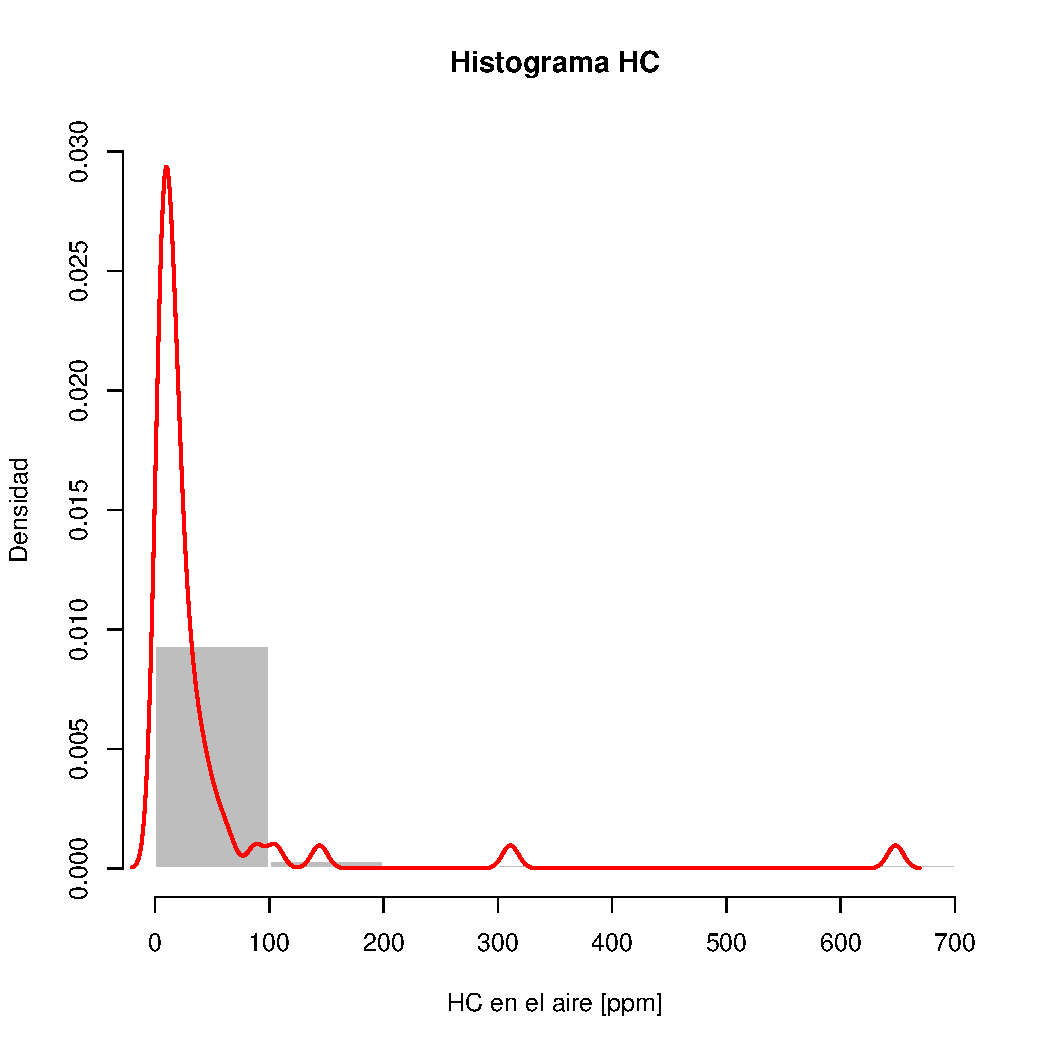
\includegraphics[width = 0.4\textwidth]{histhc}
\end{wrapfigure}

El histograma confirma el análisis anterior, muy cargado a la izquierda, puntiagudo y podemos observar los outliers de San Francisco y Los Ángeles-Long Beach. La mayoría de los datos se encuentran entre 1[ppm] y 100[ppm], esto se confirma al estudiar el boxplot de la variable.
\\
\\
\\
\\
\\
\\
\\
\\
\\
\\

\begin{wrapfigure}{l}{0.5\textwidth}
    \centering
    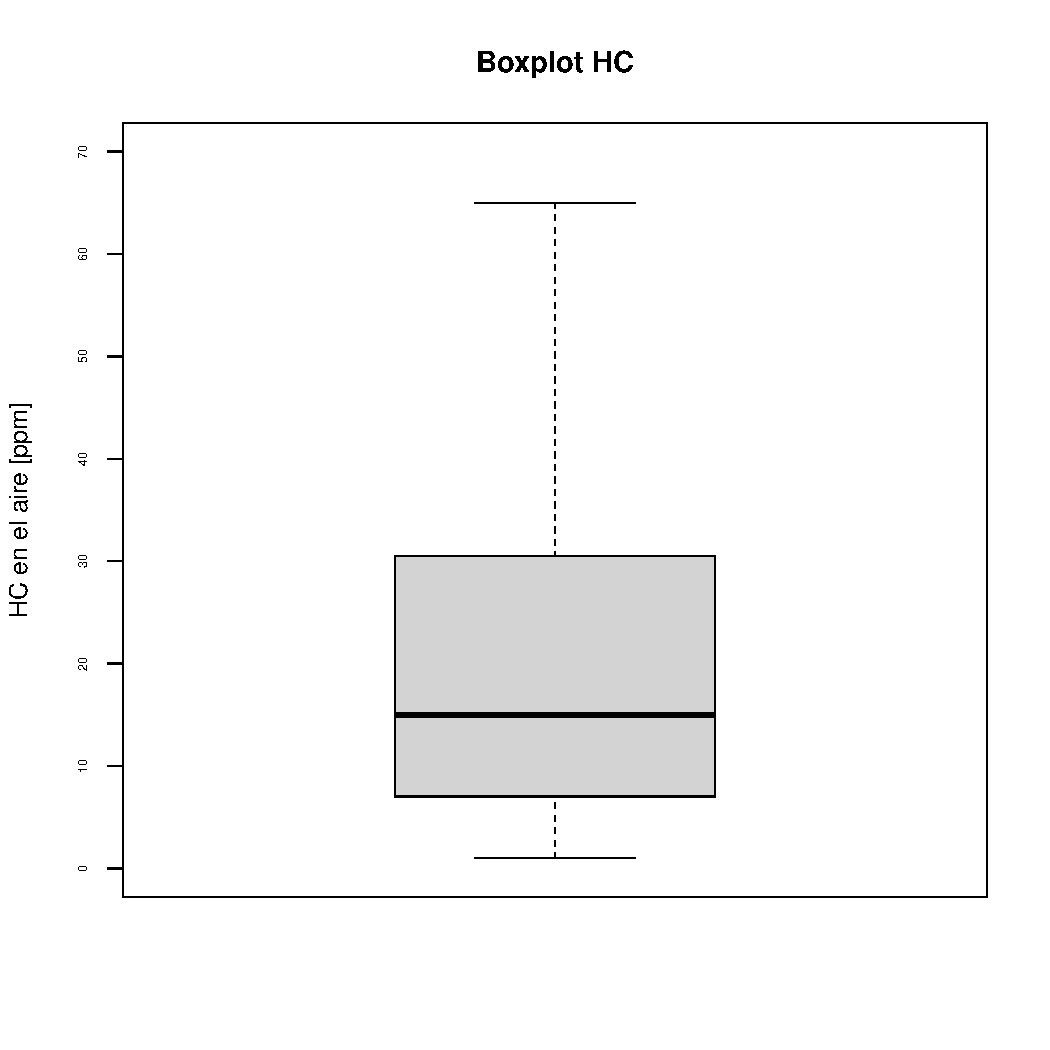
\includegraphics[width = 0.4\textwidth]{boxhc}
\end{wrapfigure}

En el boxplot de los datos, en el que no se muestran los outliers, la mayoría de mediciones se encuentra bajo los 70[ppm].

Con este análisis se desprende que la densidad de cantidades de HC se encuentra entre 1[ppm] y 70[ppm], esto debe considerarse al momento de relacionar la variable con otras, puesto que los outliers no entregan información estadísticamente concluyente.
\\
\\
\\
\\
\\
\subsubsection{SO_2}

\begin{center}
\begin{tabular}{|c|c|}
    \hline
    Variable & Unidad  \\ \hline
    SO_2 & ppm \\
    \hline
\end{tabular}
\end{center}

\textbf{Medidas descriptivas de centro:}

\begin{center}
\begin{tabular}{|c|c|c|}
    \hline
    Promedio ponderado & Mediana & Moda \\ \hline
    54.661 & 32 & 1 \\
    \hline
\end{tabular}
\end{center}

Como en los dos gases anteriores, se observa una gran diferencia entre las medidas descriptivas centrales de la variable SO_2.$ La moda es uno, por lo que este parece ser un gas menos común que los anteriores.
\\
\\
\textbf{Medidas descriptivas de posición:}

\begin{center}
\begin{tabular}{|c|c|c|c|c|}
    \hline
    Mínimo valor & Primer cuartil & Segundo cuartil & Tercer cuartil & Máximo valor\\ \hline
    1 & 13 & 32 & 70 & 278\\
    \hline
\end{tabular}
\end{center}

A pesar de las medidas de tendencia central, esta variable tiene una distribución más equitativa, según el estudio de sus cuartiles. También tiene un máximo menor al de los otros dos gases, confirmando que este aparece en menores cantidades
\\
\\
\textbf{Medidas descriptivas de dispersión y forma:}

\begin{center}
\begin{tabular}{|c|c|c|c|c|}
    \hline
    Desviación estándar  & Varianza & Skewness & Kurtosis\\ \hline
    63.5517 & 4038.814 & 1.8022 & 2.8894\\
    \hline
\end{tabular}
\end{center}

Las medidas de dispersión confirman que esta variable esta distribuida de manera más equitativa. Tiene, sin embargo, asimetría, otra vez inclinándose a la izquierda.La kurtosis es muho menor a las otras dos variables, lo que denota una concentración alrededor de la mediana también menor, un gr´áfico menos puntiagudo y más suave.
\\
\\
\textbf{Gráficos de distribución:}
\\

\begin{wrapfigure}{r}{0.5\textwidth}
    \centering
    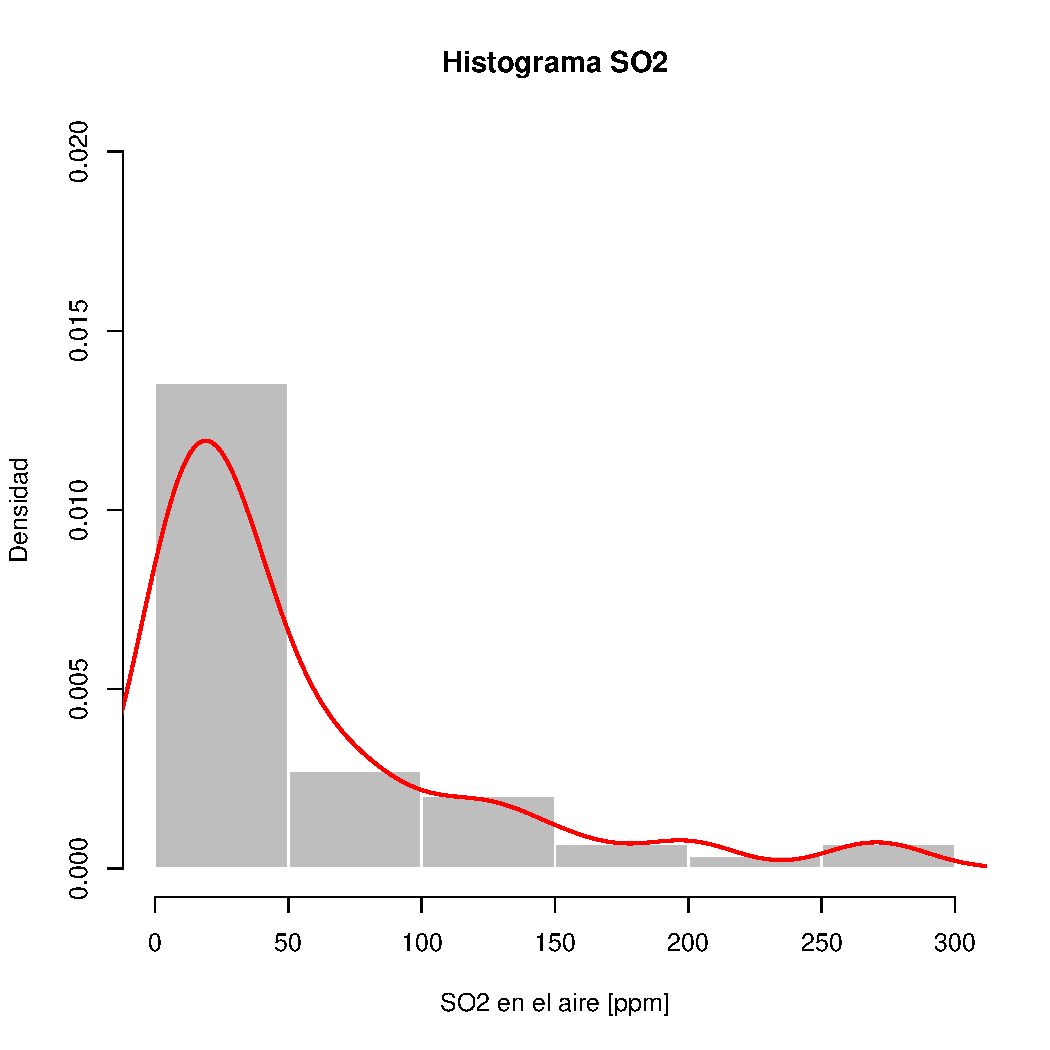
\includegraphics[width = 0.4\textwidth]{histso2}
\end{wrapfigure}

El histograma es, efectivamente, más equitativo. La kurtosis se nota menor pues la linea de densidad es mucho más suave que la de los otros dos gases. Si bien la medida de skewness resulto menor que en los otros dos, el gráfico parece estar igual de cargado a la izquierda. En realidad este valor fue menor porque el rango de valores de esta variable es menor, y los valores de la derecha son más comunes. La gran mayoría de los datos se encuentra antes de los 150[ppm].
\\
\\
\begin{wrapfigure}{l}{0.5\textwidth}
    \centering
    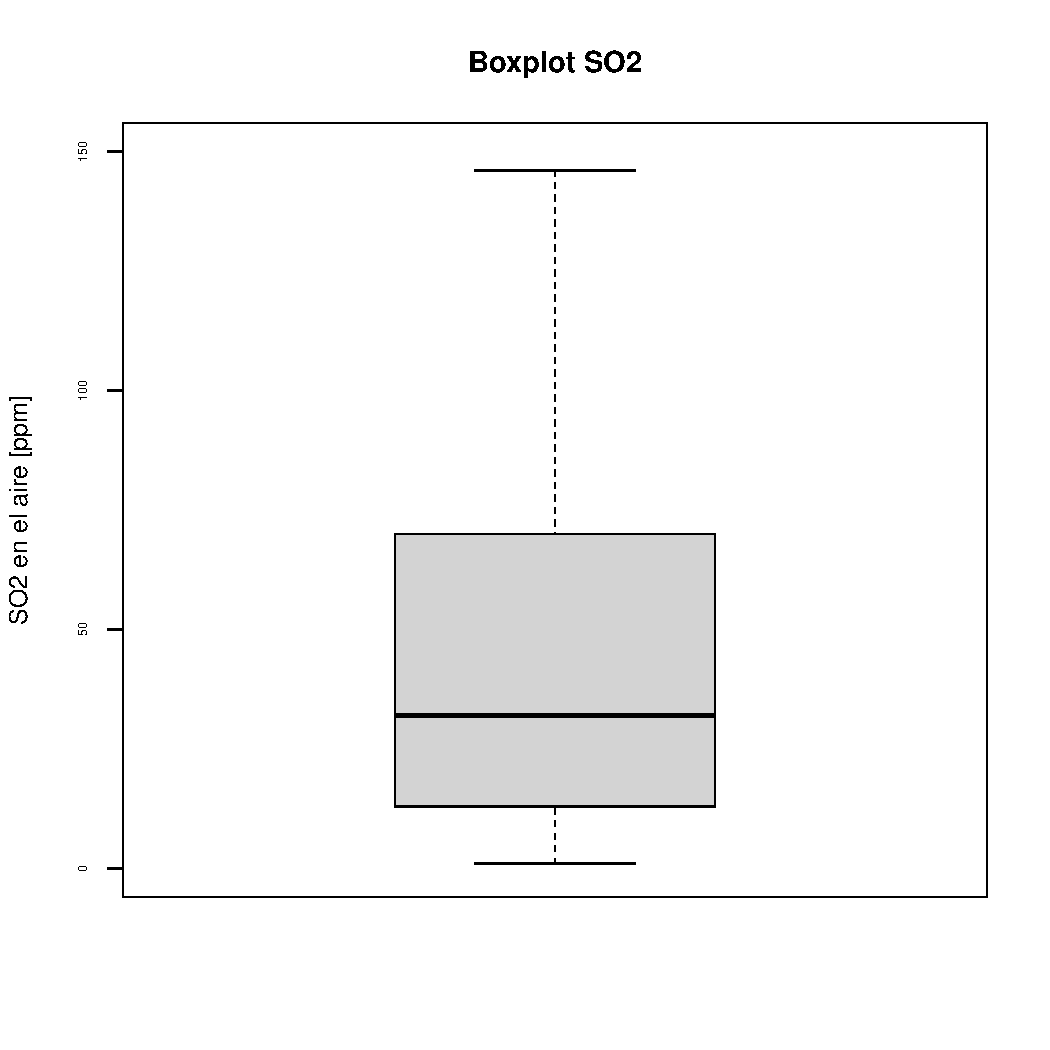
\includegraphics[width = 0.4\textwidth]{boxso2}
\end{wrapfigure}

Se confirma con el boxplot que la distribución de los valores tiene mayor densidad antes de los 150[ppm]

Las cantidades de SO_2$ son menores que las de los otros gases, y se acota su distribución más densa entre 1[ppm] y 150[ppm]. A pesar de lo anterior, los valores extremos no están tan alejados, así que de todas formas vale la pena observar su comportamiento.
\\
\\
\\
\\
\\

\subsection{Variables de población}

\subsubsection{Población total}

\begin{center}
\begin{tabular}{|c|c|}
    \hline
    Variable & Unidad  \\ \hline
    Población total & Número de personas \\
    \hline
\end{tabular}
\end{center}

\textbf{Medidas descriptivas de centro:}

\begin{center}
\begin{tabular}{|c|c|c|}
    \hline
    Promedio ponderado & Mediana & Moda \\ \hline
    1438037 & 914427 & Ninguna \\
    \hline
\end{tabular}
\end{center}

Como en los dos gases anteriores, se observa una gran diferencia entre las medidas descriptivas centrales de la variable SO_2.$ La moda es uno, por lo que este parece ser un gas menos común que los anteriores.
\\
\\
\textbf{Medidas descriptivas de posición:}

\begin{center}
\begin{tabular}{|c|c|c|c|c|}
    \hline
    Mínimo valor & Primer cuartil & Segundo cuartil & Tercer cuartil & Máximo valor\\ \hline
    1 & 13 & 32 & 70 & 278\\
    \hline
\end{tabular}
\end{center}

A pesar de las medidas de tendencia central, esta variable tiene una distribución más equitativa, según el estudio de sus cuartiles. También tiene un máximo menor al de los otros dos gases, confirmando que este aparece en menores cantidades
\\
\\
\textbf{Medidas descriptivas de dispersión y forma:}

\begin{center}
\begin{tabular}{|c|c|c|c|c|}
    \hline
    Desviación estándar  & Varianza & Skewness & Kurtosis\\ \hline
    63.5517 & 4038.814 & 1.8022 & 2.8894\\
    \hline
\end{tabular}
\end{center}

Las medidas de dispersión confirman que esta variable esta distribuida de manera más equitativa. Tiene, sin embargo, asimetría, otra vez inclinándose a la izquierda.La kurtosis es muho menor a las otras dos variables, lo que denota una concentración alrededor de la mediana también menor, un gr´áfico menos puntiagudo y más suave.
\\
\\
\textbf{Gráficos de distribución:}
\\

\begin{wrapfigure}{r}{0.5\textwidth}
    \centering
    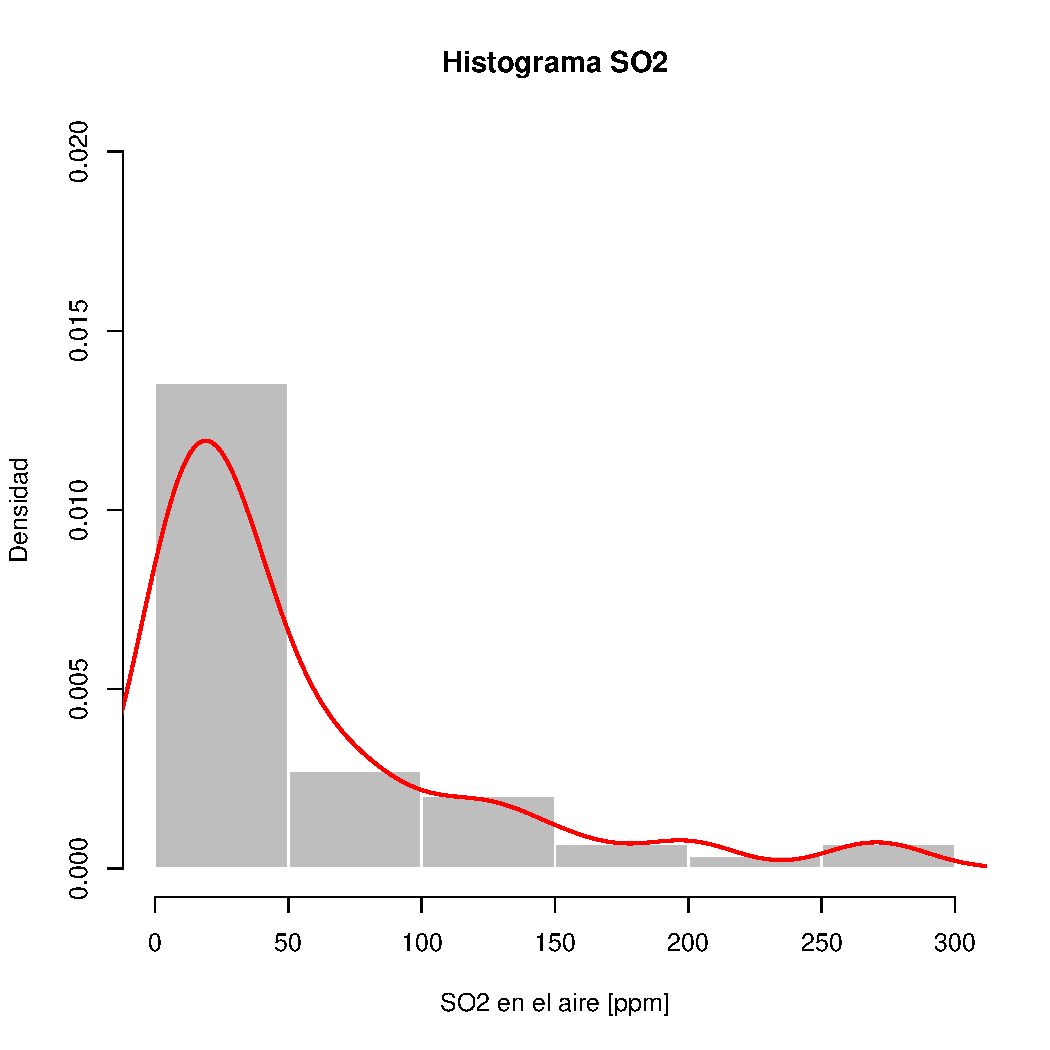
\includegraphics[width = 0.4\textwidth]{histso2}
\end{wrapfigure}

El histograma es, efectivamente, más equitativo. La kurtosis se nota menor pues la linea de densidad es mucho más suave que la de los otros dos gases. Si bien la medida de skewness resulto menor que en los otros dos, el gráfico parece estar igual de cargado a la izquierda. En realidad este valor fue menor porque el rango de valores de esta variable es menor, y los valores de la derecha son más comunes. La gran mayoría de los datos se encuentra antes de los 150[ppm].
\\
\\
\begin{wrapfigure}{l}{0.5\textwidth}
    \centering
    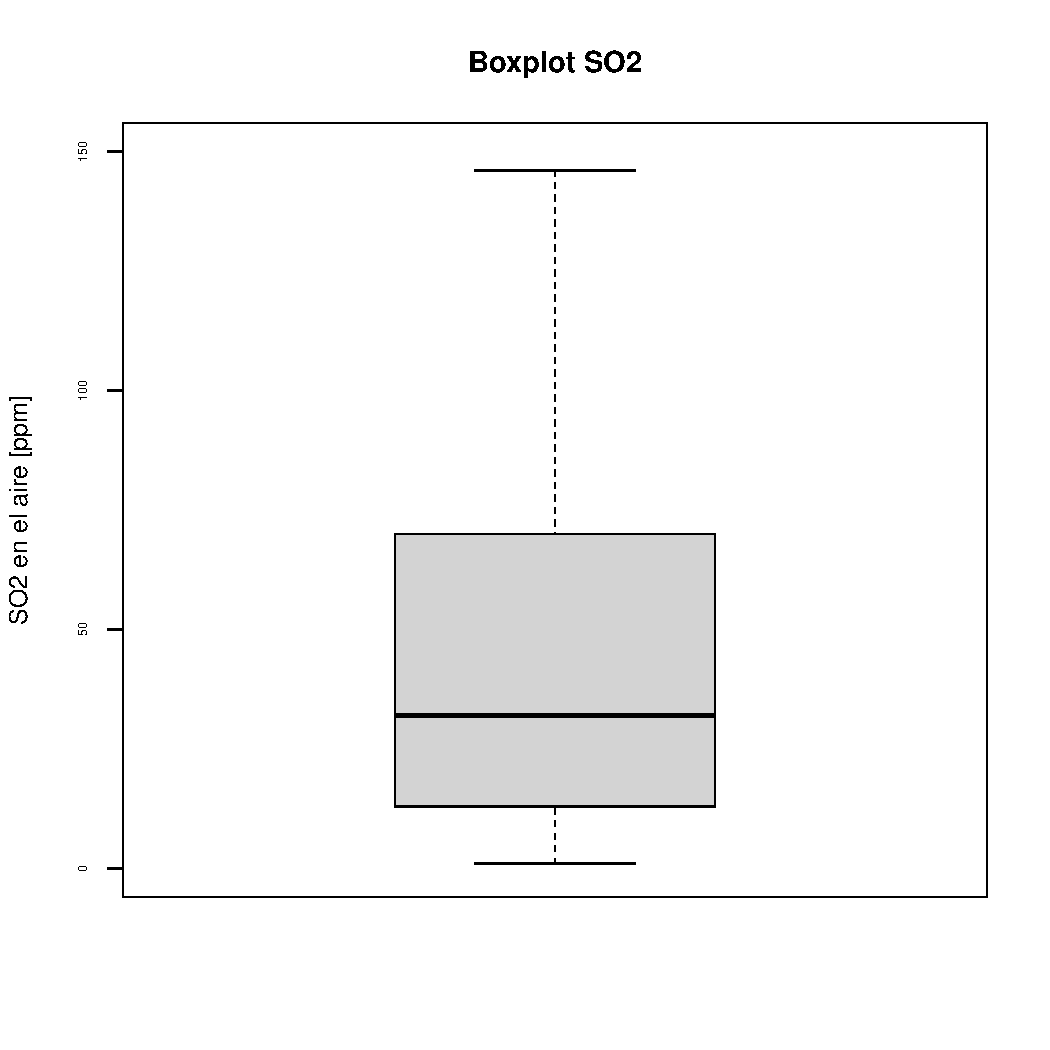
\includegraphics[width = 0.4\textwidth]{boxso2}
\end{wrapfigure}

Se confirma con el boxplot que la distribución de los valores tiene mayor densidad antes de los 150[ppm]

Las cantidades de SO_2$ son menores que las de los otros gases, y se acota su distribución más densa entre 1[ppm] y 150[ppm]. A pesar de lo anterior, los valores extremos no están tan alejados, así que de todas formas vale la pena observar su comportamiento.
\\
\\
\\
\\
\\



\section{Mortalidad y gases contaminantes}

\section{Contaminación en NY y OH}

\section{Ajuste de modelo para población por hogar}

\end{document}
